\documentclass[12pt]{article}

\usepackage{fontawesome}
\usepackage{hyperref}
\usepackage{xurl}
\usepackage{fancyvrb}
\usepackage{graphicx}
\usepackage{float}
\usepackage[tagged, highstructure]{accessibility}
\usepackage{bookmark}
\usepackage{enumitem}

\hypersetup{
    colorlinks=false,
    pdfborder={0 0 0},
    pdftitle={SQL Scaling},
    pdfauthor={Adrianna Holden-Gouveia},
    pdfsubject={Advanced Data - Lab Assignment},
    pdflang={en-US},
    pdfkeywords={SQL scaling, HackerRank, case studies, ACID transactions, scalability}
}

% Configure PDF bookmarks for navigation
\bookmarksetup{
    numbered,
    open,
}

% Configure list spacing for better accessibility
\setlist{nosep}



\title{SQL scaling}
\author{
        Adrianna Holden-Gouveia \\
        Website: \href{https://aholdengouveia.name}{aholdengouveia.name}\\ 
        \date{\vspace{-5ex}}
        %Email: \href{mailto:admin@aholdengouveia.name}{admin@aholdengouveia.name} \\
%        \faLinkedin{: aholdengouveia} \\
        \faGithub {: aholdengouveia} \\
        %\faTwitter {: aholdengouveia} \\
        }

%S\date{\today}


\begin{document}    

\maketitle

%\begin{abstract}
%This is a template for Linux Administration Lab work
%\end{abstract}
%\tableofcontents


\section*{Accessibility Notice}
This document is also available in HTML format at:

Link: \href{https://aholdengouveia.name/AdvData/labs/wk11sqlscaling.html}{\textbf{\nolinkurl{https://aholdengouveia.name/AdvData/labs/wk11sqlscaling.html}}}

The HTML version provides enhanced accessibility features including keyboard navigation, screen reader support, responsive design, dark mode support, and high contrast options.

\section*{Request}
\noindent\textbf{Request:} DATA-4630\\
\textbf{Requested by:} Head of the data team\\
\textbf{Data:} Your database, and your data collection plan from the Big Data lab

\section*{Background}
If your data collection plan goes ahead, your database is going to grow. Your manager wants to know how it would scale, how the data could be split across servers if needed, and what could go wrong for the business along the way. You'll warm up with a real business case study, then plan for your own company's growth.

\section*{Learning Outcomes}
By the end of this lab, you will be able to:
\begin{itemize}
    \item Write SQL queries to solve a real-world business case study
    \item Evaluate how a data set would scale, including vertical and horizontal scaling
    \item Choose a shard key for a data set, using queries on the data to justify it
    \item Explain how ACID transactions protect a business, and what happens when they fail
\end{itemize}

\section*{Lab Instructions}
Use your own data set and company for Parts 2 to 4. Books are my example data only.

\subsection*{Screenshots}
Several parts of this lab ask for a screenshot. Each screenshot should have your name, term, and year.  One of the easiest ways to do that is make a text document with your name and term/year on your computer and save it to use all term. Any screenshots that don't include this information won't be counted.

\begin{figure}[H]
    \centerline{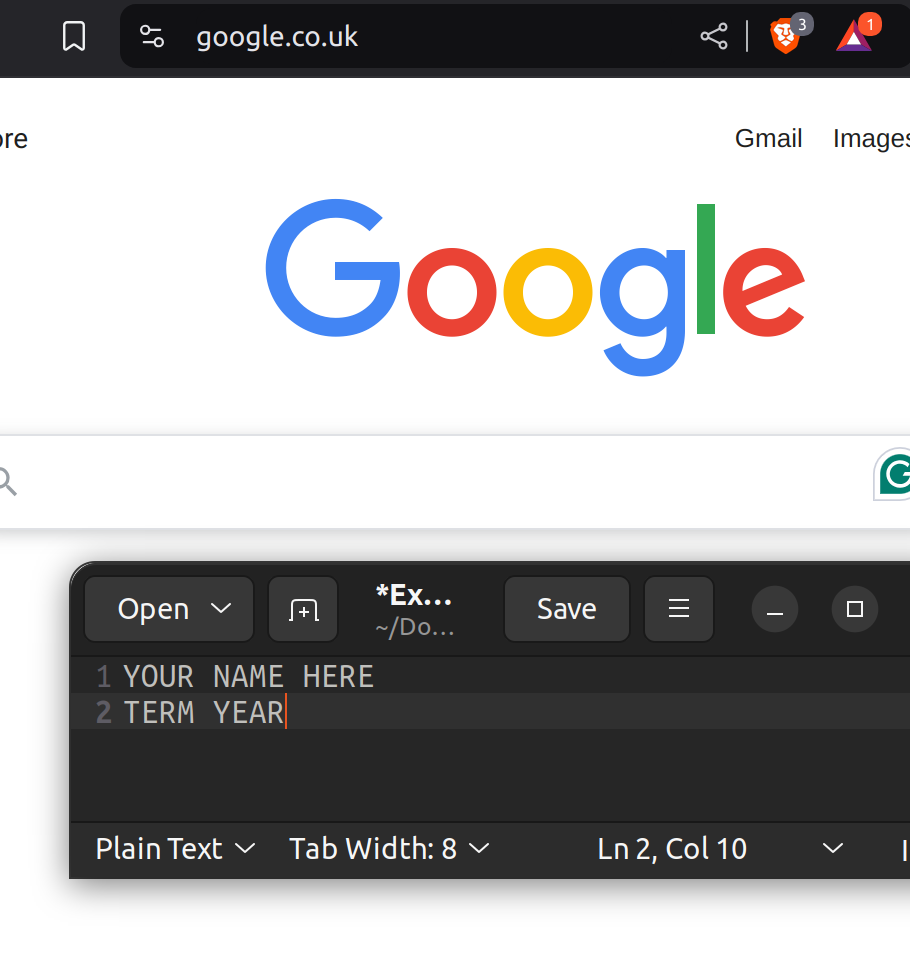
\includegraphics[scale=.2]{ExampleScreenshot.png}}
    \caption{This is an image of what each of your screenshots should look like}
    \alt{Example screenshot: a web browser showing the Google home page, with a small text editor window in front of it that says YOUR NAME HERE and TERM YEAR}
\end{figure}

\subsection*{Part 1: Case Study}
Solve all 10 questions in Case Study 1, Danny's Diner, from the 8 Week SQL Challenge (linked under Resources). Each answer should be a single SQL statement. You can use the editor on the case study page, or load the data into SandboxSQL or another tool.
\begin{enumerate}
    \item Take a screenshot of each solution and its results.
    \item With each screenshot, explain how you solved it and what resources you used. If you needed a hint, say where you found it.
\end{enumerate}
\textbf{Optional, not required for this class:} if you'd like more practice, try the Pizza Metrics questions in Case Study 2, Pizza Runner.

\subsection*{Part 2: How Would It Scale?}
\begin{enumerate}
    \item Using the estimates in your data collection plan from the Big Data lab, roughly how many rows would your database have in 1 year, and in 5 years? Show your working.
    \item The topic page explains vertical scaling, adding more power to one server, and horizontal scaling, adding more servers. Which would your company need first, and why? Think about cost, and about the size of your company.
\end{enumerate}

\subsection*{Part 3: Choose a Shard Key}
If your company ever splits its data across servers, it needs a shard key: the column that decides which server each row goes to. The topic page lists 4 things to check: cardinality, frequency, whether the values keep increasing, and query patterns.
\begin{enumerate}
    \item Pick 3 columns in your main table that could be shard keys.
    \item For each one, run these queries on your own data, replacing the table and column names, and take a screenshot of the results. The first shows the cardinality, how many different values there are. The second shows the frequency, which values appear most often.
\begin{Verbatim}
SELECT COUNT(DISTINCT genre) FROM books;

SELECT genre, COUNT(*) FROM books
GROUP BY genre
ORDER BY COUNT(*) DESC
LIMIT 5;
\end{Verbatim}
    \item For each column, explain whether its values keep increasing, like a date or an ID that goes up by one, and whether it matches the queries your company runs most, such as your documented queries from the SQL Review labs.
    \item Pick the best shard key, and explain why using your results. What data skew, where one server ends up with much more data than the others, could still happen?
\end{enumerate}
For example, in my book data, genre has only 10 different values, and 50 of my 99 books are Classics. If genre were the shard key, the server holding Classics would get half of all the data, so it would make a poor shard key.

\subsection*{Part 4: ACID and Your Business}
Pick one real transaction your company would make, such as a sale that records the payment and updates the stock.
\begin{enumerate}
    \item For each of the 4 ACID properties, atomicity, consistency, isolation, and durability, explain what it means for this transaction, and what would go wrong for the business if it failed.
    \item Which property matters most to your company, and why?
    \item Would splitting your data across servers make that property harder to keep? Why or why not?
\end{enumerate}

\section*{Acceptance Criteria}
This request is done when:
\begin{itemize}
    \item All 10 Danny's Diner questions are solved with single SQL statements, each with a screenshot and an explanation
    \item Your growth estimates for 1 and 5 years show your working, and your choice of vertical or horizontal scaling is explained
    \item 3 possible shard keys are checked with queries on your own data, with screenshots
    \item Your shard key choice is justified using your results, including any data skew that could still happen
    \item All 4 ACID properties are explained for a real transaction at your company
    \item Every screenshot follows the screenshot rules
\end{itemize}

\section*{Deliverables}
One file that includes Parts 1 to 4.

Audience: the head of the data team.

\section*{Resources}
References, a video, a PowerPoint and some notes are available at my website
Link: \href{https://www.aholdengouveia.name/AdvData/SQLscaling.html}{\textbf{\nolinkurl{https://www.aholdengouveia.name/AdvData/SQLscaling.html}}}

Case Study 1, Danny's Diner
Link: \href{https://8weeksqlchallenge.com/case-study-1/}{\textbf{\nolinkurl{https://8weeksqlchallenge.com/case-study-1/}}}

Optional: Case Study 2, Pizza Runner
Link: \href{https://8weeksqlchallenge.com/case-study-2/}{\textbf{\nolinkurl{https://8weeksqlchallenge.com/case-study-2/}}}

Suggested tool: SandboxSQL, free, runs in your browser, and saves your database as a file with its Export button
Link: \href{https://www.sandboxsql.com/}{\textbf{\nolinkurl{https://www.sandboxsql.com/}}}

\end{document}